%===============================================================================
% LaTeX sjabloon voor de bachelorproef toegepaste informatica aan HOGENT
% Meer info op https://github.com/HoGentTIN/latex-hogent-report
%===============================================================================

\documentclass[dutch,dit,thesis]{hogentreport}

% TODO:
% - If necessary, replace the option `dit`' with your own department!
%   Valid entries are dbo, dbt, dgz, dit, dlo, dog, dsa, soa
% - If you write your thesis in English (remark: only possible after getting
%   explicit approval!), remove the option "dutch," or replace with "english".

\usepackage{lipsum} % For blind text, can be removed after adding actual content

%% Pictures to include in the text can be put in the graphics/ folder
\graphicspath{{graphics/}}

%% For source code highlighting, requires pygments to be installed
%% Compile with the -shell-escape flag!
\usepackage[section]{minted}
\usemintedstyle{solarized-light}
\definecolor{bg}{RGB}{253,246,227} %% Set the background color of the codeframe

%% Change this line to edit the line numbering style:
\renewcommand{\theFancyVerbLine}{\ttfamily\scriptsize\arabic{FancyVerbLine}}

%% Macro definition to load external java source files with \javacode{filename}:
\newmintedfile[javacode]{java}{
    bgcolor=bg,
    fontfamily=tt,
    linenos=true,
    numberblanklines=true,
    numbersep=5pt,
    gobble=0,
    framesep=2mm,
    funcnamehighlighting=true,
    tabsize=4,
    obeytabs=false,
    breaklines=true,
    mathescape=false
    samepage=false,
    showspaces=false,
    showtabs =false,
    texcl=false,
}

% Other packages not already included can be imported here

%%---------- Document metadata -------------------------------------------------
% TODO: Replace this with your own information
\author{Arno Ooms}
\supervisor{Dhr. Verschraege}
\cosupervisor{Dhr. J. Roels}
\title[Optionele ondertitel]%
    {Het beveiligen van containers in een Kubernetes cluster: onderzoek en proof of concept.}
\academicyear{\advance\year by -1 \the\year--\advance\year by 1 \the\year}
\examperiod{1}
\degreesought{\IfLanguageName{dutch}{Professionele bachelor in de toegepaste informatica}{Bachelor of applied computer science}}
\partialthesis{false} %% To display 'in partial fulfilment'
%\institution{Internshipcompany BVBA.}

%% Add global exceptions to the hyphenation here
\hyphenation{back-slash}

%% The bibliography (style and settings are  found in hogentthesis.cls)
\addbibresource{bachproef.bib}            %% Bibliography file
\addbibresource{../voorstel/voorstel.bib} %% Bibliography research proposal
\defbibheading{bibempty}{}

%% Prevent empty pages for right-handed chapter starts in twoside mode
\renewcommand{\cleardoublepage}{\clearpage}

\renewcommand{\arraystretch}{1.2}

%% Content starts here.
\begin{document}

%---------- Front matter -------------------------------------------------------

\frontmatter

\hypersetup{pageanchor=false} %% Disable page numbering references
%% Render a Dutch outer title page if the main language is English
\IfLanguageName{english}{%
    %% If necessary, information can be changed here
    \degreesought{Professionele Bachelor toegepaste informatica}%
    \begin{otherlanguage}{dutch}%
       \maketitle%
    \end{otherlanguage}%
}{}

%% Generates title page content
\maketitle
\hypersetup{pageanchor=true}

%%=============================================================================
%% Voorwoord
%%=============================================================================

\chapter*{\IfLanguageName{dutch}{Woord vooraf}{Preface}}%
\label{ch:voorwoord}

%% TODO:
%% Het voorwoord is het enige deel van de bachelorproef waar je vanuit je
%% eigen standpunt (``ik-vorm'') mag schrijven. Je kan hier bv. motiveren
%% waarom jij het onderwerp wil bespreken.
%% Vergeet ook niet te bedanken wie je geholpen/gesteund/... heeft

%%=============================================================================
%% Samenvatting
%%=============================================================================

% TODO: De "abstract" of samenvatting is een kernachtige (~ 1 blz. voor een
% thesis) synthese van het document.
%
% Een goede abstract biedt een kernachtig antwoord op volgende vragen:
%
% 1. Waarover gaat de bachelorproef?
% 2. Waarom heb je er over geschreven?
% 3. Hoe heb je het onderzoek uitgevoerd?
% 4. Wat waren de resultaten? Wat blijkt uit je onderzoek?
% 5. Wat betekenen je resultaten? Wat is de relevantie voor het werkveld?
%
% Daarom bestaat een abstract uit volgende componenten:
%
% - inleiding + kaderen thema
% - probleemstelling
% - (centrale) onderzoeksvraag
% - onderzoeksdoelstelling
% - methodologie
% - resultaten (beperk tot de belangrijkste, relevant voor de onderzoeksvraag)
% - conclusies, aanbevelingen, beperkingen
%
% LET OP! Een samenvatting is GEEN voorwoord!

%%---------- Nederlandse samenvatting -----------------------------------------
%
% TODO: Als je je bachelorproef in het Engels schrijft, moet je eerst een
% Nederlandse samenvatting invoegen. Haal daarvoor onderstaande code uit
% commentaar.
% Wie zijn bachelorproef in het Nederlands schrijft, kan dit negeren, de inhoud
% wordt niet in het document ingevoegd.

\IfLanguageName{english}{%
\selectlanguage{dutch}
\chapter*{Samenvatting}
\lipsum[1-4]
\selectlanguage{english}
}{}

%%---------- Samenvatting -----------------------------------------------------
% De samenvatting in de hoofdtaal van het document

\chapter*{\IfLanguageName{dutch}{Samenvatting}{Abstract}}

\lipsum[1-4]


%---------- Inhoud, lijst figuren, ... -----------------------------------------

\tableofcontents

% In a list of figures, the complete caption will be included. To prevent this,
% ALWAYS add a short description in the caption!
%
%  \caption[short description]{elaborate description}
%
% If you do, only the short description will be used in the list of figures

\listoffigures

% If you included tables and/or source code listings, uncomment the appropriate
% lines.
%\listoftables
%\listoflistings

% Als je een lijst van afkortingen of termen wil toevoegen, dan hoort die
% hier thuis. Gebruik bijvoorbeeld de ``glossaries'' package.
% https://www.overleaf.com/learn/latex/Glossaries

%---------- Kern ---------------------------------------------------------------

\mainmatter{}

% De eerste hoofdstukken van een bachelorproef zijn meestal een inleiding op
% het onderwerp, literatuurstudie en verantwoording methodologie.
% Aarzel niet om een meer beschrijvende titel aan deze hoofdstukken te geven of
% om bijvoorbeeld de inleiding en/of stand van zaken over meerdere hoofdstukken
% te verspreiden!

%%=============================================================================
%% Inleiding
%%=============================================================================

\chapter{\IfLanguageName{dutch}{Inleiding}{Introduction}}%
\label{ch:inleiding}

Kubernetes is een snel opkomende en krachtige opensourcesoftware voor het automatiseren en beheren van containers. Deze containers kunnen Docker of een andere technologie zijn. Om deze containers te laten communiceren en samenwerken, worden deze toegepast binnen een Kubernetes cluster. 

De scope van dit onderzoek omvat de belangrijkste zaken die te maken hebben met Docker containers te beveiligen binnen een Kubernetes cluster. De configuratie van de applicaties binnen deze containers zijn niet van toepassing in deze paper. In dit onderzoek worden tools zoals kubehunter en kube-bench besproken voor het analyseren en het uitvoeren van beveiligings validaties. 

%De inleiding moet de lezer net genoeg informatie verschaffen om het onderwerp te begrijpen en in te zien waarom de onderzoeksvraag de moeite waard is om te onderzoeken. In de inleiding ga je literatuurverwijzingen beperken, zodat de tekst vlot leesbaar blijft. Je kan de inleiding verder onderverdelen in secties als dit de tekst verduidelijkt. Zaken die aan bod kunnen komen in de inleiding~\autocite{Pollefliet2011}:

%\begin{itemize}
%  \item context, achtergrond
%  \item afbakenen van het onderwerp
%  \item verantwoording van het onderwerp, methodologie
%  \item probleemstelling
%  \item onderzoeksdoelstelling
%  \item onderzoeksvraag
%  \item \ldots
%\end{itemize}

\section{\IfLanguageName{dutch}{Probleemstelling}{Problem Statement}}%
\label{sec:probleemstelling}

Securex, een sociaal zekerings bedrijf gevestigd in gent, maakt gebruik van een Kubernetes omgeving met Docker containers om hun applicaties te laten draaien. Een belangrijk aspect van het gebruik van deze containers is de beveiliging ervan. Zonder effectieve beveiligingsmaatregelen en isolatie van de containers en de Kubernetes omgeving kunnen deze containers blootgesteld worden aan beveiligingsrisico's. Als deze containers gevoelige informatie bevatten kan dit erge gevolgen hebben voor Securex.

%Uit je probleemstelling moet duidelijk zijn dat je onderzoek een meerwaarde heeft voor een concrete doelgroep. De doelgroep moet goed gedefinieerd en afgelijnd zijn. Doelgroepen als ``bedrijven,'' ``KMO's'', systeembeheerders, enz.~zijn nog te vaag. Als je een lijstje kan maken van de personen/organisaties die een meerwaarde zullen vinden in deze bachelorproef (dit is eigenlijk je steekproefkader), dan is dat een indicatie dat de doelgroep goed gedefinieerd is. Dit kan een enkel bedrijf zijn of zelfs één persoon (je co-promotor/opdrachtgever).

\section{\IfLanguageName{dutch}{Onderzoeksvraag}{Research question}}%
\label{sec:onderzoeksvraag}

\begin{itemize}
    \item Wat is kubernetes? Waarin speelt kubernetes een belangrijker rol?
    \item Wat zijn de kwetsbaarheden van kubernetes?
    \item Wat zijn drie belangrijke tools of oplossingen tegen deze kwetsbaarheden? Waarin verschillen deze oplossingen of tools?
    \item Zijn er tools beschikbaar die software kan scannen die geïnstalleerd word op kubernetes?
    \item Zijn er tools of oplossingen beschikbaar om configuratie van kubernetes te valideren?
\end{itemize}
%Wees zo concreet mogelijk bij het formuleren van je onderzoeksvraag. Een onderzoeksvraag is trouwens iets waar nog niemand op dit moment een antwoord heeft (voor zover je kan nagaan). Het opzoeken van bestaande informatie (bv. ``welke tools bestaan er voor deze toepassing?'') is dus geen onderzoeksvraag. Je kan de onderzoeksvraag verder specifiëren in deelvragen. Bv.~als je onderzoek gaat over performantiemetingen, dan 

\section{\IfLanguageName{dutch}{Onderzoeksdoelstelling}{Research objective}}%
\label{sec:onderzoeksdoelstelling}

Securex verwacht dat de beveiliging van een Docker container in een Kubernetes omgeving zo volledig mogelijk in kaart wordt gebracht. Dit houdt in dat de verschillende tools, bedreigingen en oplossingen uitvoerig onderzocht worden. Het resultaat van dit onderzoek zal Securex in staat stellen om hun containers beter te isoleren en beschermen tegen bedreigingen en beveiligingsrisico's.
%Wat is het beoogde resultaat van je bachelorproef? Wat zijn de criteria voor succes? Beschrijf die zo concreet mogelijk. Gaat het bv.\ om een proof-of-concept, een prototype, een verslag met aanbevelingen, een vergelijkende studie, enz.

\section{\IfLanguageName{dutch}{Opzet van deze bachelorproef}{Structure of this bachelor thesis}}%
\label{sec:opzet-bachelorproef}

% Het is gebruikelijk aan het einde van de inleiding een overzicht te
% geven van de opbouw van de rest van de tekst. Deze sectie bevat al een aanzet
% die je kan aanvullen/aanpassen in functie van je eigen tekst.

De rest van deze bachelorproef is als volgt opgebouwd:

In Hoofdstuk~\ref{ch:stand-van-zaken} wordt een overzicht gegeven van de stand van zaken binnen het onderzoeksdomein, op basis van een literatuurstudie.

In Hoofdstuk~\ref{ch:methodologie} wordt de methodologie toegelicht en worden de gebruikte onderzoekstechnieken besproken om een antwoord te kunnen formuleren op de onderzoeksvragen.

% TODO: Vul hier aan voor je eigen hoofstukken, één of twee zinnen per hoofdstuk
In Hoofdstuk~\ref{ch:methodologie} wordt een proof-of-concept gemaakt om de literatuurstudie technischer te bespreken.

In Hoofdstuk~\ref{ch:conclusie}, tenslotte, wordt de conclusie gegeven en een antwoord geformuleerd op de onderzoeksvragen. Daarbij wordt ook een aanzet gegeven voor toekomstig onderzoek binnen dit domein.
\chapter{\IfLanguageName{dutch}{Stand van zaken}{State of the art}}%
\label{ch:stand-van-zaken}

% Tip: Begin elk hoofdstuk met een paragraaf inleiding die beschrijft hoe
% dit hoofdstuk past binnen het geheel van de bachelorproef. Geef in het
% bijzonder aan wat de link is met het vorige en volgende hoofdstuk.

% Pas na deze inleidende paragraaf komt de eerste sectiehoofding.
\section{Definities}

\begin{itemize}
    \item \textit{Container: Een container is een standaard software-eenheid die code en al zijn afhankelijkheden verpakt, zodat de toepassing snel en betrouwbaar van de ene computeromgeving naar de andere draait \autocite{Docker-2023}. Containers zijn lichtgewicht en bevatten alles wat nodig is om de applicatie te draaien, dus u hoeft niet te vertrouwen op wat er momenteel op de host is geïnstalleerd. \autocite{DockerDocs-2023} }
    \item \textit{Docker: Docker biedt de mogelijkheid om een aplicatie te verpakken en uit te voeren in een geïsoleerde omgeving, genaamd een container.  \autocite{DockerDocs-2023} }
\end{itemize}

\ref{fig:KubernetesContainers} Geeft een beter beeld wat containers zijn en welke functie docker heeft.

\begin{flushleft}
    \begin{figure}[h]
        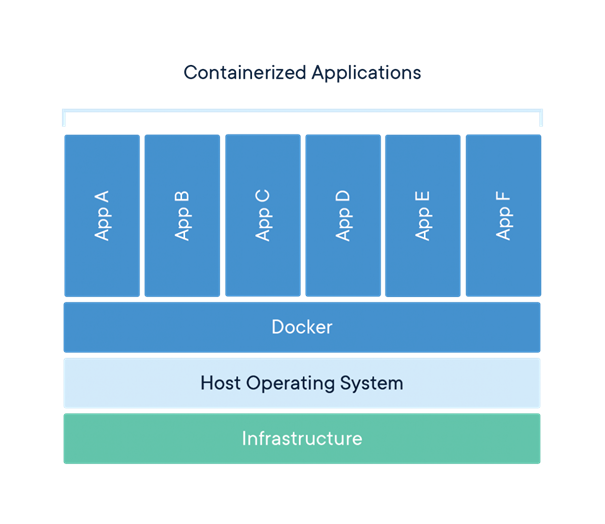
\includegraphics[width=.49\textwidth]{graphics/container.png}
        \caption{\label{fig:KubernetesContainers}Container architectuur \autocite{Docker-2023}}
    \end{figure} 
\end{flushleft}

\section{Kubernetes}
Kubernetes, ook wel afgekort als K8s, is een gratis en open-source systeem dat wordt gebruikt om de implementatie, schaling en het beheer van containerapplicaties te automatiseren \autocite{KubernetesDocs-2023}. 
Het biedt de mogelijkheid om containers die deel uitmaken van een applicatie te groeperen en te beheren als logische eenheden, waardoor het gemakkelijk wordt om deze te ontdekken en te beheren \autocite{KubernetesDocs-2023}.
Docker is een containerisatieplatform, terwijl Kubernetes een orkestratietool is voor het beheer van meerdere containers.
Docker biedt een eenvoudige en efficiënte methode voor het aanmaken en inzetten van containers, terwijl Kubernetes complexere functionaliteit biedt voor het beheer van containers op schaal \autocite{banerjee-2023}.
Voor grotere, complexere projecten die uitgebreid containerbeheer vereisen, is Kubernetes een krachtiger en flexibeler hulpmiddel.

\subsection{Kubernetes Componenten - Overview}
\autocite{KubernetesDocs-2023} Bij het ontplooien van kubernetes ontstaat er een cluster. Een cluster bestaat uit een groep machines zogenaamd \textit{worker nodes}. Zo een node heeft verschillende componenten zoals een Kubelet, een kube-proxy en een container-runtime.
Binnen deze worker nodes zijn er pods met containers in. In deze containers kunnen applicaties zoals een SQL database of een website draaien. 
\autocite{KubernetesDocs-2023} Binnen een cluster is er ook een control plane die de globale beslissingen neemt over bijvoorbeeld scheduling of een pod starten. De control plane beheert ook de nodes. 
\autocite{KubernetesDocs-2023} Een control plane bestaat uit verschillende componenten zoals een Kube-apiserver, etcd, kube-scheduler en een kube-controller-manager. 
De kube-apiserver is een belangrijk component van de control plane want deze is verantwoordelijk voor de communicatie van gebruikers, de cluster en externe componenten \autocite{hohn-2020}. 
De kubernetes API laat toe om de staat van objecten zoals pods, namespaces te manipuleren \autocite{KubernetesDocs-2023}.
De etcd binnen een control plane is een key value opslagplaats voor alle data van de cluster, het is belangrijk dat ten alle tijde deze data beschermd is van ongewilde manipulatie \autocite{KubernetesDocs-2023}. 
Om voor fouttolerantie en hoge beschikbaarheid te zorgen, draait de control plane in productiescenario's meestal op vele machines, en een cluster bevat doorgaans meerdere nodes \autocite{KubernetesDocs-2023}. 
In leer- of middelenbeperkte omgevingen is er meestal maar één node aanwezig.

\subsubsection{Pod}
Een pod is een groep van één of meer containers \autocite{habbal-2020}.
Alle containers in een pod delen hetzelfde IP adres en dezelfde middelen zoals volumes \autocite{hohn-2020}.
In makkelijkere woorden is een pod een enkele instantie van een applicatie die kan worden gerepliceerd als er meer instanties nodig zijn om de toenemende druk op te vangen \autocite{habbal-2020}.
Gerepliceerde pods zijn creëert en beheert als een groep door de middelen en de control plane \textcite{KubernetesDocs-2023}.

\subsubsection{Service}
\textit{Een service is een methode om een netwerktoepassing die als een of meer Pods in uw cluster draait, bloot te stellen \autocite{KubernetesDocs-2023}.}

\subsubsection{Namespace}
Een namespace dient om objecten te organiseren in een cluster.
Een soort folder die objecten houd \autocite{burns-2022}.

\subsubsection{Kubelet}
De kubelet is het belangrijkste component dat op elke node aanwezig is \autocite{Vayghan2019}.
Kubelet draait de Docker-containers die aan zijn node zijn toegewezen, voert regelmatig gezondheidscontroles op ze uit, en rapporteert hun status en die van de node aan de master \autocite{Vayghan2019}.

\subsubsection{Volume}
Een volume maakt het mogelijk om opslag te delen tussen de containers in een pod, of tussen pods op dezelfde node \autocite{Baier2017}.

\subsubsection{ConfigMap}
De ConfigMap binnen kubernetes is een soort volume en een middel voor het opslaan van configuratie data \autocite{KubernetesDocs-2023}.
Het is een manier om configuratie data te injecteren in pods \autocite{KubernetesDocs-2023}.

\subsubsection{Kubectl}
Kubectl is een commmand-line tool om opdrachten, ook wel commando's genoemd, te kunnen uitvoeren op de control plane van de cluster.
Deze command-line tool maakt gebruik van de Kubernetes API \autocite{KubernetesDocs-2023}.

\begin{flushleft}
    \begin{figure}[h]
        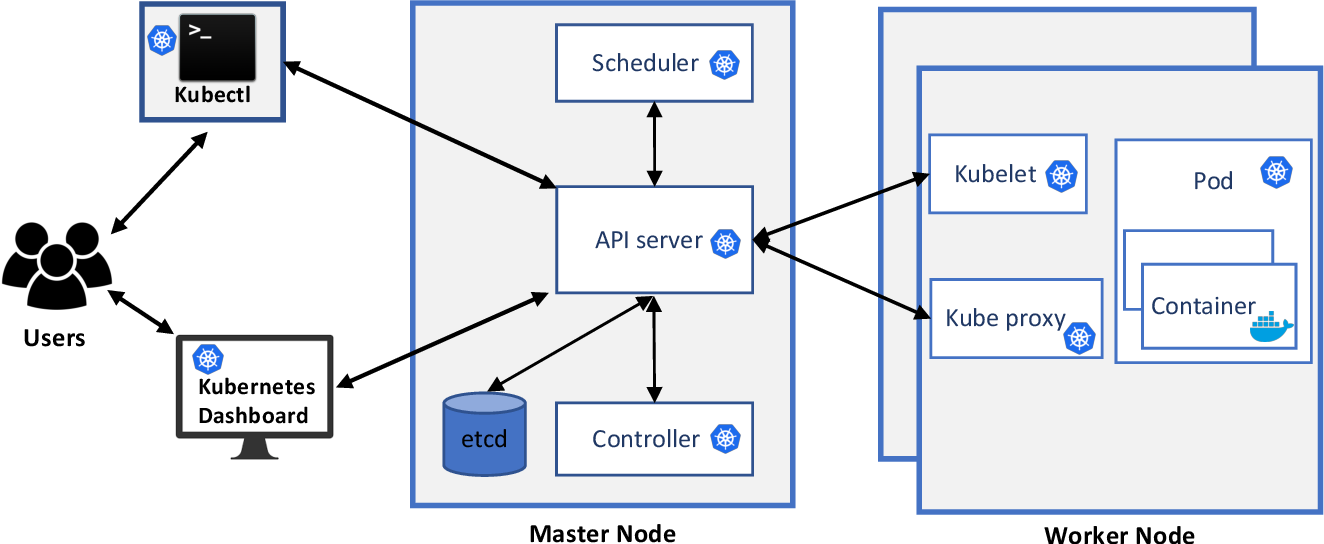
\includegraphics[width=.70\textwidth]{graphics/3-Figure1-1.png}
        \caption{\label{fig:KubernetesOverview}Deze afbeelding geeft een duidelijk overzicht van de componenten van kubernetes en hoe ze met elkaar interacteren.  \autocite{shamim2020xi}}
    \end{figure} 
\end{flushleft}


\section{Kwetsbaarheden}

\subsection{Misconfiguratie}
Een studie in 2023 van \textcite{red-hat-2023} toont aan dat 45 percent van DevOps ingenieurs een veiligheidsincident heeft ervaren die te maken heeft met de misconfiguratie van containers en/of clusters. Pods in een Kubernetes-cluster kunnen standaard met elkaar communiceren, door deze communicatie ontstaan er veiligheidslekken als het niet goed is geconfigureerd. De grootste bezorgdheid rond misconfiguratie is het blootstellen van gevoelige informatie \autocite{red-hat-2023}. Andere soorten veiligheids misconfiguraties dat de ingenieurs zich zorgen om maken zijn ongepatchte fouten, het behoud van de standaard configuratie, errors in de code en containers met foute rechten. \newline

Vaak voorkomende misconfiguratie fouten kunnen tot grote problemen voor een applicatie zorgen. Namelijk 40 percent zijn het meest bezorgd dat er ransomware aanvallen gebeuren als kubernetes of de containers niet juist zijn geconfigureerd en 53 percent hebben al een ransomware aanval ervaren in de laatste 12 maanden \autocite{red-hat-2023}. De meest voorkomende aanval bij misconfiguraties is een Denial of service (DoS) attack \autocite{red-hat-2023}. Een DoS aanval heeft als doel het systeem onbruikbaar of ontoegankelijk te maken voor de gebruikers. \newline

Standaard configuratie binnen de kubernetes cluster kan leiden tot anonieme niet-geauthenticeerde gebruikers om kwaadaardige activiteiten uit te voeren. Een kwaadwillende gebruiker kan bijvoorbeeld de standaardinstellingen voor een onbeveiligde toegang achterhalen, toegang krijgen tot de control plane en schadelijke commando's uitvoeren \autocite{shamim2020xi}.

\subsection{etcd}
Als een aanvaller toegang krijgt tot de etcd, kan de aanvaller potentiële toegang tot gevoelige data verkrijgen of de staat van de cluster aanpassen of data aanpassen. Fout geconfigureerde etcd instellingen kunnen de database open zetten tot aanvallen van buitenaf en ongewilde toegang \autocite{KubernetesDocs-2023}.

\subsection{API server}
Via de kubectl command is het mogelijk om API requests naar de server te sturen om middelen en workloads te beheren \autocite{KubernetesDocs-2023}. Iedereen die schrijf rechten heeft of iedereen die toegang heeft tot de Kubernetes API kan de cluster controleren \autocite{KubernetesDocs-2023}. 
Standaard zal de API server luisteren naar poort 6443 \autocite{KubernetesDocs-2023}. Iedereen die toegang krijgt tot het systeem waar de master op draait, heeft volledige toegang tot de cluster \autocite{Rice2018}. \newline

\subsection{RBAC}
RBAC (Rolgebaseerde toegangscontrole) is het concept dat machtigingen worden geassocieerd met rollen, en dat gebruikers lid worden van de juiste rollen, waardoor zij de machtigingen van de rollen verkrijgen \autocite{Sandhu1998}. Doordat misconfiguraties niet vanaf een centrale locatie kunnen worden gedetecteerd, hersteld en voorkomen, kunnen clusters worden gecompromitteerd \autocite{OWASP-2023}. Volgens de top 10 Kubernetes risico's van OWASP in 2022 is RBAC de derde meest gevaarlijke risico. RBAC is de primaire authorisatie methode voor Kubernetes en is verantwoordelijk van de permissies over de middelen en componenten \autocite{OWASP-2023}. Er bestaat een 'superuser' binnen kubernetes genaamd cluster-admin. Deze cluster-admin heeft toegang om elke actie uit te voeren op elke component binnen een Kubernetes cluster \autocite{OWASP-2023}. 

RBAC wordt gebruikt om elk verzoek dat binnenkomt op de API-server goed te keuren of te weigeren \autocite{mytilinakis2020attack}. Als een gebruiker een API request maakt naar het eindpunt zonder enige authenticatie dan is hij geassocieerd met als een anonieme gebruiker \autocite{mytilinakis2020attack}. Het mogelijk maken van anonieme toegang naar eindpunten kan ook de waarschijnlijkheid van het vrijgeven van gevoelige informatie verhogen \autocite{Rice2018}. Het is onwaarschijnlijk dat deze informatie iets belangrijks in gevaar brengt, maar het kan de aanvaller de weg wijzen naar andere zwakheden \autocite{Rice2018}.

\subsection{Supply chain}
35 percent van de respondenten in de studie van \textcite{red-hat-2023} zijn het meest bezorgd over kwetsbaarheden in de software gerelateerd aan de software supply chain. Een software supply chain is de verzameling van de componenten, softwares, tools die gebruikt worden om een applicatie te bouwen. Hierbij komen open-source softwares aanbod en het gebruik hiervan creëren uitdagingen in de beveiliging van de applicatie \autocite{red-hat-2023}. Kwetsbaarheden in software kunnen leiden tot grote beveiligingsproblemen, zoals datalekken, malware-infecties en onbevoegde toegang \autocite{shamim2020xi}. De bedrijven van de correspondenten zijn het meest bezorgd in kwetsbare componenten van een applicatie, onvoldoende toegang controle en een tekort aan Software Bill of Materials (SBOM) of herkomst \autocite{red-hat-2023}. Deze studie toont ook aan dat bijna 70 percent van de correspondenten al problemen hebben gehad met een kwetsbare CI/CD pipeline en kwetsbare componenten in de applicatie. \newline

Containers en docker images horen ook tot software supply chain. Containers kunnen kwetsbaarheden en schadelijke software bevatten. Als er zwakheden in een Kubernetes-cluster zitten, wordt het hele container-orkestratiesysteem, evenals de meegeleverde apps, kwetsbaar voor aanvallen \autocite{shamim2020xi}. Als de images en deployment-configuraties van Kubernetes-componenten niet worden gecontroleerd, kan het Kubernetes-cluster vatbaar worden voor onbevoegde gebruikers. Wanneer deze images worden uitgerold, kunnen aanvallers toegang krijgen en gebruikmaken van zwakke plekken \autocite{shamim2020xi}. \newline

Volgens \textcite{OWASP-2023} zijn er drie belangrijke termen binnen de kwetsbaarheden van supply chain:
\begin{itemize}
    \item Image Integrity: Dit verwijst naar de zekerheid van een container image. De zekerheid dat de image is wat het beweert te zijn, dat het geen kwaadaardige code bevat en dat het in geen enkele wijze aangepast is \autocite{OWASP-2023}. 
    \item Image Composition: Een container image is opgemaakt uit verschillende lagen. Elke laag representeert bepaalde veiligheidsimplicaties. Container images met onbelangrijke software kunnen gebruikt worden om privileges te verhogen of kwetsbaarheden uit te buiten \autocite{OWASP-2023}. 
    \item Bekende software kwetsbaarheden: Vele container images gebruiken paketten van derde partijen die kwetsbaarheden kunnen bevatten die uitgebuit kunnen worden. Als docker images kwetsbare versies van software bevatten kan dit de kubernetes cluster in gevaar brengen \autocite{OWASP-2023}. 
\end{itemize}


\subsection{Container runtime}
In het onderzoek van \textcite{red-hat-2023} toont aan dat 49 percent van de gerelateerde veiligheidsincidenten in kubernetes of containers gebeuren via beveiligingsincidenten tijdens runtime. De container runtime is een van de meest kritische componenten in een kubernetes cluster \autocite{mytilinakis2020attack}. De container runtime dat in dit onderzoek wordt gebruikt is Docker, de meest voorkomende. Docker heeft zelf veiligheidsinstellingen en functies. Kwetsbaarheden in containers kunnen leiden tot het in gevaar brengen van andere componenten. 

\subsection{Images}
In de sectie van \textit{Software supply chain} wordt er al een klein stukje besproken over images. Images worden meestal uit een publieke plaats gedownload. Het is dus mogelijk dat deze docker images niet altijd de juiste intenties hebben en mogelijks kwade bedoelingen hebben en kwetsbaarheden veroorzaken \autocite{mytilinakis2020attack}. 

\subsection{Kubernetes API server}
\paragraph{Statische pods}
Volgens \textcite{KubernetesDocs-2023} is er een risico bij statische pods waarbij aanvallers statische pods kunnen wijzigen of nieuwe statische pods kunnen toevoegen waardoor API-serverconroles worden omzeild. 
Dit risco kan worden veroorzaakt door foute schrijfrechten toe te kennen tot de locatie waar statische pods zijn opgeslagen.

\paragraph{Kubelet API}
De kubelet API biedt een HTTP API dat informatie vrijgeeft over de draaiende pods, pod logs en staat het uitvoeren van commando's in containers toe.
Directe toegang tot de Kubelet API omzeilt toegangscontrole en is niet gelogd door Kubernetes audit logging.


\section{Tools en oplossingen}

\subsection{misconfiguratie}
Deze sectie bespreekt algemeen advies hoe de configuratie kan verbetert worden en bespreekt ook verschillende tools voor het verifiëren van de configuratie.\newline

Om beveiliging in te stellen op een pod kan dit met het veld \textit{securityContext} in de specificatie van de pod. \textit{securityContext} is een \textit{PodSecurityContext} object \autocite{KubernetesDocs-2023}. 
Deze beveiligingsinstellingen gelden voor alle containers binnen de pod \autocite{KubernetesDocs-2023}. 
Volgens \textcite{OWASP-2023} is een proces als root gebruiker draaien een vaak voorkomende fout. Voor sommige workloads is de root gebruiker een vereiste maar het is aangeraden om het te vermijden. Als de container met root rechten gecompromitteerd wordt dan zou de aanvaller root rechten hebben om schadelijke acties te kunnen uitvoeren \autocite{OWASP-2023}.  

Een ander voorbeeld van \textcite{OWASP-2023} beschrijft dat het aangeraden is om read-only (alleen-lees) bestandssystemen te gebruiken. Alleen-lees bestandssystemen limiteren de impact van een gecompromitteerde container op een kubernetes node \autocite{OWASP-2023}. Dit zorgt ervoor dat een kwaadaardig proces het host systeem niet kan herschrijven of aanpassen.

Volgens \textcite{OWASP-2023} is het aangeraden om containers zonder privileges te draaien. De container kan verdere middelen of capaciteiten krijgen als de container als privilege draait. 

Deze drie voorbeelden kunnen allemaal vermeden worden in de configuratie van een pod. Dit is bij de sectie 'securitycontext'. 
\begin{minted}{console}
    apiVersion: v1  
    kind: Pod  
    metadata:  
    name: root-priviliged-readOnly
    spec:  
    containers:  
    ...
    securityContext:  
    #Privileges staan aan 
    privileged: true
    #root gebruiker staat aan
    runAsUser: 0
    #De container runned als een gebruiker en niet als root
    runAsUser: 5554
    #alleen-lees rechten zijn geconfigureerd
    readOnlyRootFilesystem: true
\end{minted}

Het is ook mogelijk om dit als runtime te configureren en niet in de configuratie. De applicatie kan deze miconfiguratie mitigeren door volgende maatregelen te nemen \autocite{OWASP-2023}:
\begin{itemize}
    \item Draai als niet-root gebruiker: Standaard draaien containers in Kubernetes als de root-gebruiker, die onbeperkte toegang heeft tot het systeem. Het draaien van containers als een niet-rootgebruiker kan de impact van potentiële beveiligingskwetsbaarheden helpen beperken door het niveau van toegang dat de container heeft tot het onderliggende systeem te verlagen \autocite{OWASP-2023}.
    \item Uitvoeren als niet-privilege modus: Standaard hebben containers in Kubernetes geprivilegieerde toegang tot het hostsysteem, wat betekent dat ze acties kunnen uitvoeren die de beveiliging van het systeem in gevaar kunnen brengen. Het draaien van containers in niet-privilege modus kan dit helpen voorkomen door de acties die de container kan uitvoeren te beperken \autocite{OWASP-2023}.
    \item Stel AllowPrivilegeEscalation op \textit{False}: Deze instelling verbiedt dat kindprocessen meer privileges krijgen dan hun ouderprocessen. Het voorkomt de escalatie van privileges binnen de container, wat beveiligingsproblemen kan helpen voorkomen \autocite{OWASP-2023}.
\end{itemize}

\subsubsection{Toegang tot Kubernetes API}
Kubectl maakt contact met de API server via REST calls. Bij zo een REST call naar de API, gaat de API door verschillende stadia \autocite{KubernetesDocs-2023}: 
\begin{itemize}
    \item Transport beveiliging
    \item Authenticatie
    \item Autorisatie
    \item Toegangscontrole
\end{itemize}
\paragraph{Transport beveiliging}
Het is belangrijk dat de API server niet naar een poort luistert die kwetsbaar is zoals poort 8080. Volgens \autocite{KubernetesDocs-2023} is de standaard poort 6443. Om zeker te zijn is het mogelijk om te checken op welke poort de api server draait door het commando:
\begin{minted}{console}
    kubectl config view --minify -o jsonpath='{.clusters[0].cluster.server}'
\end{minted}

De API is veilig geconfigureerd als de URL eindigt met poort 443, 8443 of 6443. Het aangeraden om dit te veranderen naar poort 6443, 8443 of 443 als de poort geconfigureerd is op 8080. Dit is mogelijk met het commando:
\begin{minted}{console}
    kube-apiserver --secure-port <port>
\end{minted}

Om bovenstaand commando uit te voeren is het nodig om kube-apiserver te installeren. 
Bovenstaand commando zal de URL geven van de kubernetes API sever. Om te verifiëren dat de poort open is kan dat met een curl commando \autocite{Rice2018}:
\begin{minted}{console}
    curl <IP address>:<port>
\end{minted}

Bij het maken van een API verzoek of REST call wordt er ook een certificaat gepresenteerd. Zo een certificaat kan ondertekent zijn door een certificate authority (CA) of een PKI (public key infrastructure) die connectie heeft met een gekende CA. Het certificaat en de private sleutel kunnen gewijzigd worden door gebruik te maken van volgende commando's \autocite{KubernetesDocs-2023}:
\begin{minted}{console}
    kube-apiserver --tsl-cert-file
    kube-apiserver --tls-private-key-file
\end{minted}

\paragraph{Authenticatie}
Eens dat er een veilige transport methode is toegepast kijkt de API naar authenticatie. Authenticatie kan plaatsvinden via clientcertificaten, wachtwoorden, tokens, serviceaccounts. Meerdere authenticatiemethoden kunnen worden ingesteld en geprobeerd.
Als een API verzoek niet kan worden geauthenticeerd dan is het verzoek geweigerd met de HTTP status code 401 \autocite{KubernetesDocs-2023}.  

\paragraph{Autorisatie}
Geauthenticeerde verzoeken moeten worden geautoriseerd. Een verzoek moet een gebruikersnaam, actie en object van de actie bevatten. Het verzoek is geautoriseerd als het niet wordt geweigerd en de gebruiker toegang heeft om die actie uit te voeren \autocite{KubernetesDocs-2023}.
Kubernetes maakt gebruik van meerdere authorisatiemethodes zoals ABAC, RBAC en Webhook mode \autocite{KubernetesDocs-2023}. 

\paragraph{Toegangscontrole}
Toegangscontrolemodules kunnen verzoeken wijzigen of weigeren. Toegangscontrolemodules zijn softwaremodules die verzoeken kunnen wijzigen of weigeren. Deze modules   handelen verzoeken af die objecten creëren, wijzigen, verwijderen of verbinden. 


\subsubsection{RBAC}


\subsubsection{Tools of middelen}






%%=============================================================================
%% Methodologie
%%=============================================================================

\chapter{\IfLanguageName{dutch}{Methodologie}{Methodology}}%
\label{ch:methodologie}

%% TODO: Hoe ben je te werk gegaan? Verdeel je onderzoek in grote fasen, en
%% licht in elke fase toe welke stappen je gevolgd hebt. Verantwoord waarom je
%% op deze manier te werk gegaan bent. Je moet kunnen aantonen dat je de best
%% mogelijke manier toegepast hebt om een antwoord te vinden op de
%% onderzoeksvraag.

\lipsum[21-25]



% Voeg hier je eigen hoofdstukken toe die de ``corpus'' van je bachelorproef
% vormen. De structuur en titels hangen af van je eigen onderzoek. Je kan bv.
% elke fase in je onderzoek in een apart hoofdstuk bespreken.

%\input{...}
%\input{...}
%...

%%=============================================================================
%% Conclusie
%%=============================================================================

\chapter{Conclusie}%
\label{ch:conclusie}

% TODO: Trek een duidelijke conclusie, in de vorm van een antwoord op de
% onderzoeksvra(a)g(en). Wat was jouw bijdrage aan het onderzoeksdomein en
% hoe biedt dit meerwaarde aan het vakgebied/doelgroep? 
% Reflecteer kritisch over het resultaat. In Engelse teksten wordt deze sectie
% ``Discussion'' genoemd. Had je deze uitkomst verwacht? Zijn er zaken die nog
% niet duidelijk zijn?
% Heeft het onderzoek geleid tot nieuwe vragen die uitnodigen tot verder 
%onderzoek?

Het beveiligen van een Kubernetes-omgeving is een complexe taak die vraagt om het gebruik van diverse (open source) tools om de beveiligingskwaliteit te waarborgen. Bij het zoeken naar oplossingen voor beveiliging is het raadzaam te vertrouwen op de officiële documentatie, aangezien Kubernetes voortdurend evolueert en de beveiliging daarmee ook verandert. Door op de hoogte te blijven van recente ontwikkelingen en best practices binnen het uitgebreide Kubernetes-ecosysteem, kunnen organisaties hun beveiligingsstrategie optimaliseren en zich effectief verdedigen tegen nieuwe bedreigingen. De CVE database is een betrouwbare database van kwetsbaarheden die essentieel is voor het identificeren en aanpakken van beveiligingsrisico's. Tools zoals kube-linter en Trivy die zich baseren op de CVE database kunnen snel en efficiënt beveiligingsrisico's vinden, al blijven recente kwetsbaarheden gemeld in de CVE database een risico voor het systeem. Daarom is het belangrijk om als organisatie regelmatig updates en patches uit te voeren om de beveiliging van het systeem up-to-date te houden. Daarnaast is het essentieel om proactief te zijn en gebruik te maken van aanvullende beveiligingsmaatregelen, zoals scannen op malware, virussen of het monitoren en detecteren van het systeem bij onbekende toegang. Het beheren van beveiligingsrisico's is een continu proces dat aandacht en toewijding vereist om de integriteit en vertrouwelijkheid van systemen en gegevens te waarborgen. Zolang de tools onderhouden worden, blijven deze een cruciale rol hebben. Trivy is een must-have tool om de beveiliging te optimaliseren. Deze tool is ontworpen en onderhouden door Aqua Security, een betrouwbaar bedrijf dat zich focust op het verstrekken van beveiligingsoplossingen. Trivy detecteert en scant alles van misconfiguraties, tot sofware supply chain en container images. Deze tool heeft de mogelijkheid om misconfiguraties te scannen en hier oplossingen voor te geven, maar KubeLinter is gespecialiseerd in het ontdekken van misconfiguraties en sneller en efficiënter in het scannen van files en geeft een duidelijke weergave voor de misconfiguraties en de oplossingen. Zowel Kube-bench als Trivy zijn essentiële tools voor het scannen van een Kubernetes-cluster. Kube-bench biedt betere prestaties in vergelijking met Trivy en geeft ook duidelijkere informatie over de gedetecteerde kwetsbaarheden, inclusief mogelijke oplossingen. Daarnaast is OPA Gatekeeper een waardevolle tool om beleidsregels te implementeren en zo misconfiguraties en kwetsbaarheden te voorkomen bij het implementeren van Kubernetes-objecten. Uit dit onderzoek is echter gebleken dat de combinatie van tools, zoals Kube-bench, Trivy en kube-linter, de beste oplossing biedt voor een effectieve beveiliging van een Kubernetes-cluster. Door gebruik te maken van deze tools kunnen zowel de prestaties, gedetailleerde informatie over kwetsbaarheden als naleving van best practices worden verbeterd. Daarnaast kan het implementeren van OPA Gatekeeper als aanvullende tool bijdragen aan het handhaven van beleidsregels en het voorkomen van misconfiguraties en kwetsbaarheden tijdens de implementatie van Kubernetes-objecten. Het gebruik van deze tools in combinatie omvatten een breed scala aan tactieken en technieken die worden beschreven in de \textit{MITRE ATT\&CK} matrix.


%---------- Bijlagen -----------------------------------------------------------

\appendix

\chapter{Onderzoeksvoorstel}

Het onderwerp van deze bachelorproef is gebaseerd op een onderzoeksvoorstel dat vooraf werd beoordeeld door de promotor. Dat voorstel is opgenomen in deze bijlage.

%% TODO: 
%\section*{Samenvatting}

% Kopieer en plak hier de samenvatting (abstract) van je onderzoeksvoorstel.

% Verwijzing naar het bestand met de inhoud van het onderzoeksvoorstel
%---------- Inleiding ---------------------------------------------------------

\section{Introductie}%
\label{sec:introductie}

Kubernetes is een snel opkomende en krachtige opensourcesoftware voor het automatiseren en beheren van containers. Deze containers kunnen Docker of een andere technologie zijn. Om deze containers te laten communiceren en samenwerken, worden deze toegepast binnen een Kubernetes cluster. 

Een Kubernetes cluster, ook wel een k8s genoemd, is een groep van noden. Deze groep noden bestaan uit minstens één master node en een aantal worker nodes. Binnen deze worker nodes zijn er pods waarin containers draaien. \textit{Figuur 1} brengt hier meer duidelijkheid over. Deze containers bevatten applicaties zoals een SQL database of een website die draait met nginx. In de literatuurstudie wordt dit uitgebreid besproken.

De scope van dit onderzoek omvat alles wat te maken heeft met Docker containers te beveiligen binnen een Kubernetes cluster. De configuratie van de applicaties binnen deze containers zijn niet van toepassing in deze paper. In dit onderzoek worden tools zoals kubehunter en kube-bench besproken voor het analyseren en het uitvoeren van beveiligings checks. 


Hoe scherm je het best een container af van bedreigingen of aanvallen? Elke laag binnen een node, zoals een pod en een container moet geïsoleerd en beschermd zijn tegen aanvallen en bedreigingen.

Hoe kan een container direct beveiligd zijn bij een deployment?

Tot hoe ver kan men gaan bij het scannen en analyseren van Docker images in een pipeline?

\begin{flushleft}
    \begin{figure}[h]
        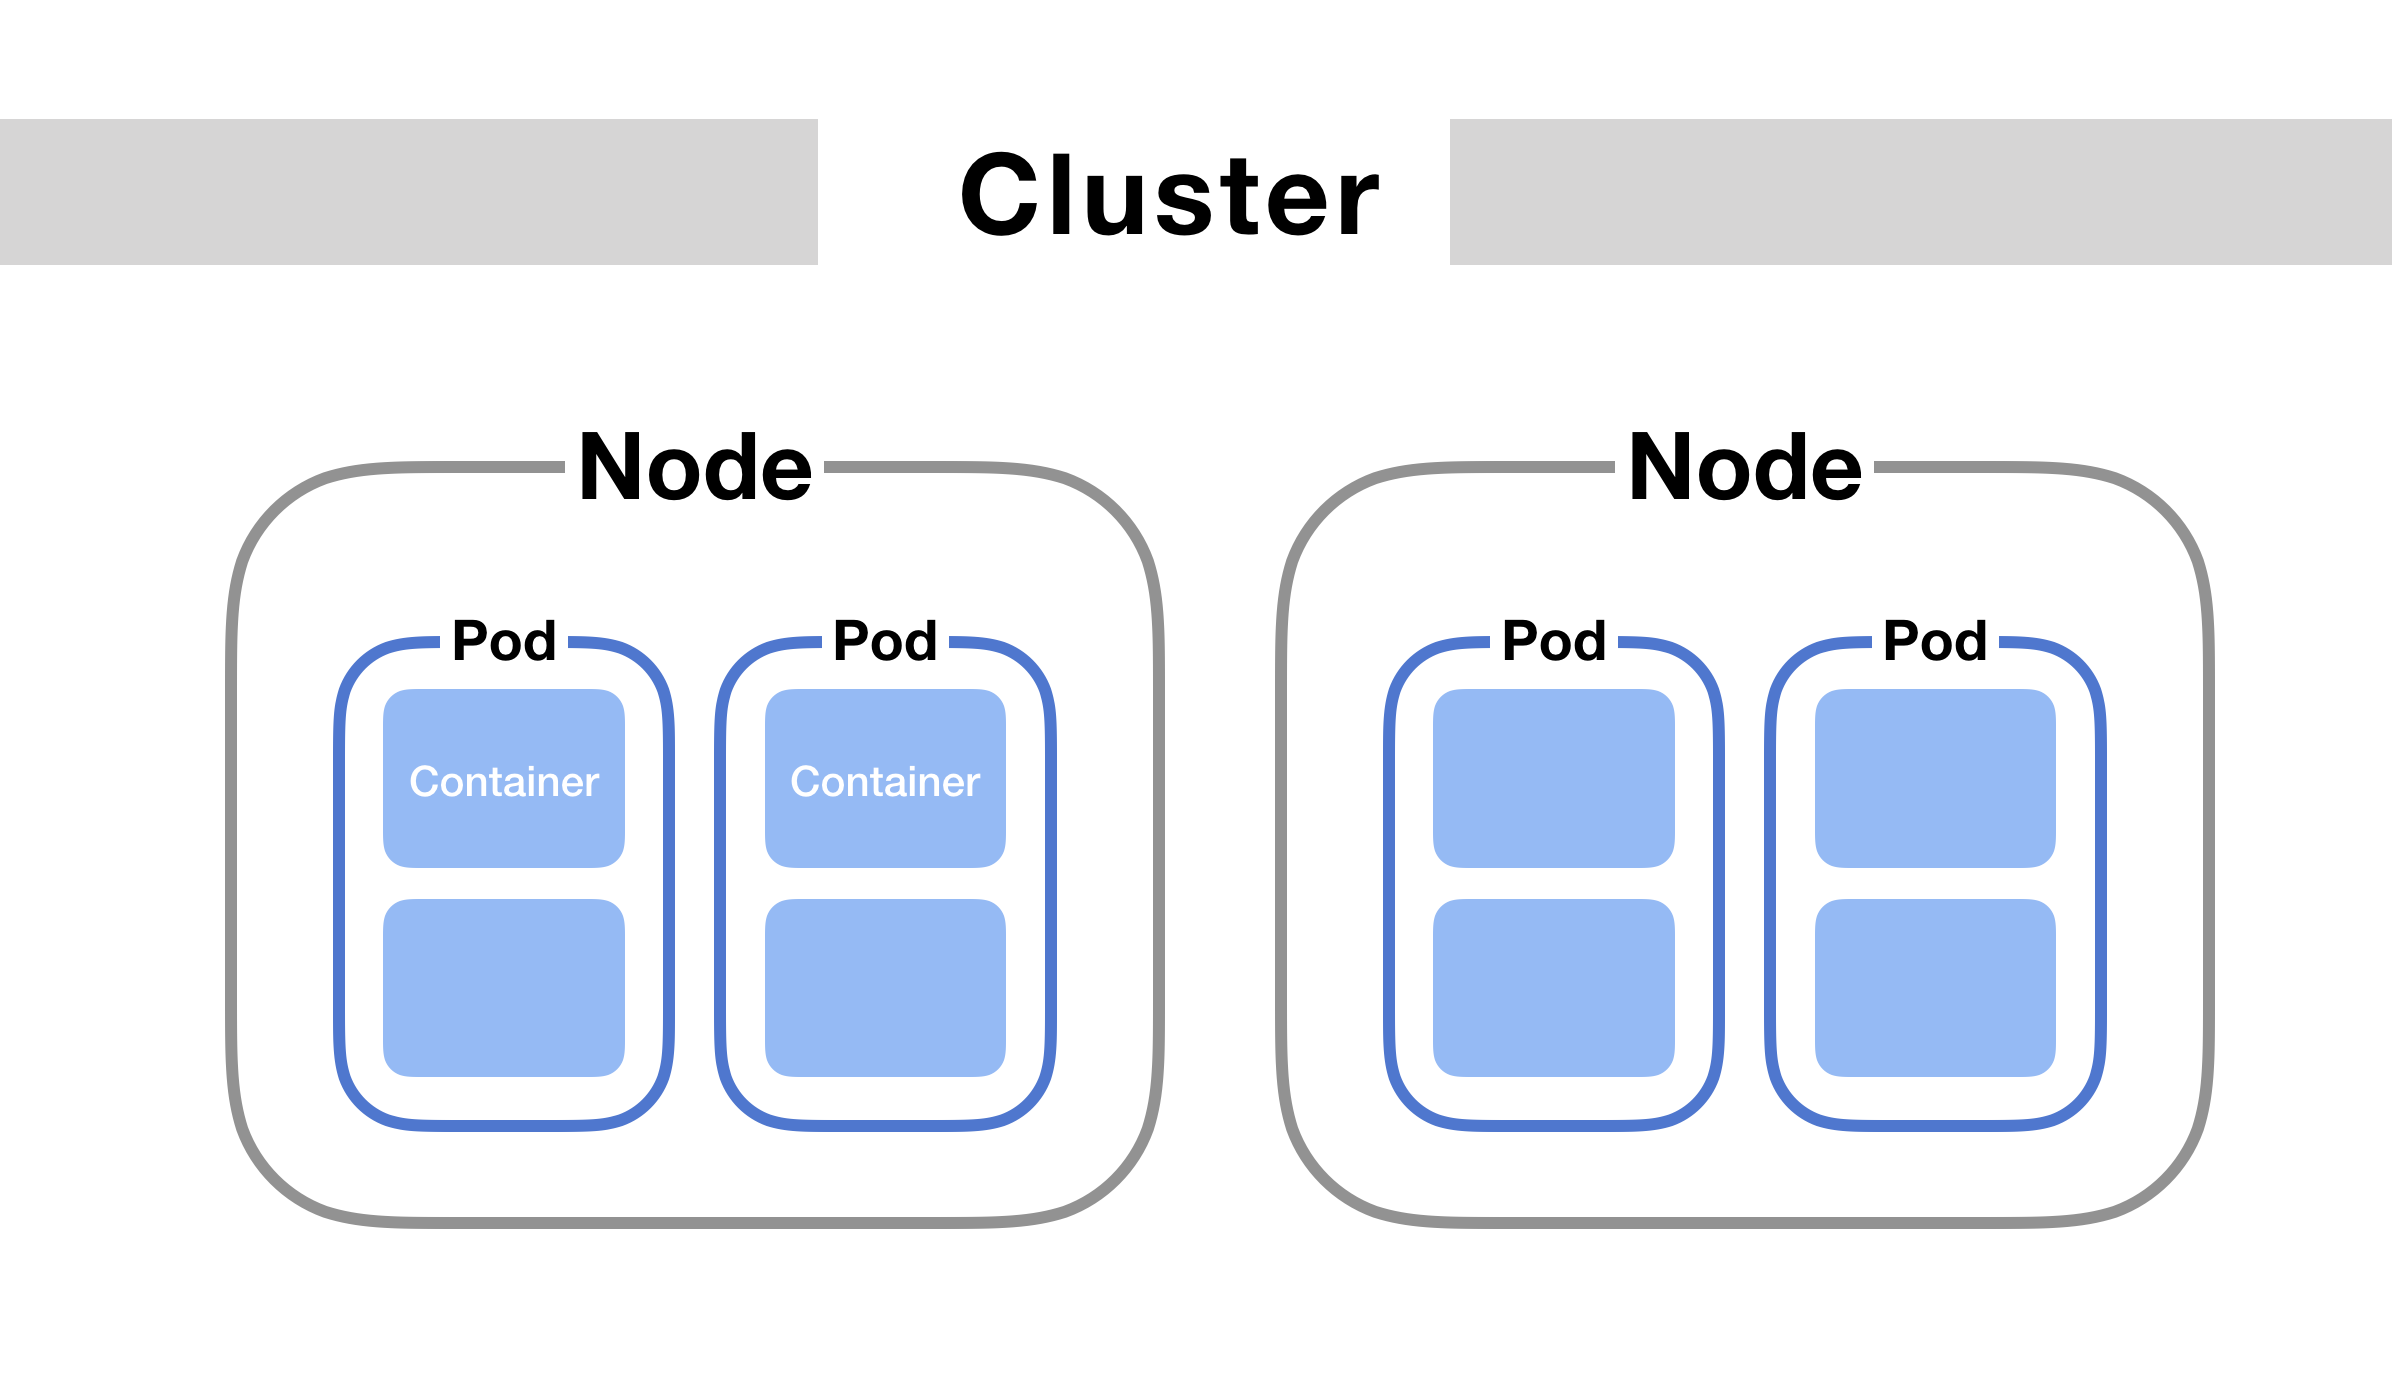
\includegraphics[width=.49\textwidth]{img/node-overview.png}
        \caption{\label{fig:Kubernetes 4c}Kubernetes cluster with nodes \autocite{kubernetes-MP}}
    \end{figure} 
\end{flushleft}

Securex, een sociaal zekerings bedrijf gevestigd in gent, maakt gebruik van een Kubernetes omgeving met Docker containers om hun applicaties te laten draaien. Een belangrijk aspect van het gebruik van deze containers is de beveiliging ervan. Zonder effectieve beveiligingsmaatregelen en isolatie van de containers en de Kubernetes omgeving kunnen deze containers blootgesteld worden aan beveiligingsrisico's. Als deze containers gevoelige informatie bevatten kan dit erge gevolgen hebben voor Securex.

Securex verwacht dat de beveiliging van een Docker container in een Kubernetes omgeving zo volledig mogelijk in kaart wordt gebracht. Dit houdt in dat de verschillende tools, bedreigingen en oplossingen uitvoerig onderzocht worden. Het resultaat van dit onderzoek zal Securex in staat stellen om hun containers beter te isoleren en beschermen tegen bedreigingen en beveiligingsrisico's.


%---------- Stand van zaken ---------------------------------------------------

\section{Literatuurstudie}%
\label{sec:Literatuurstudie}

\autocite{Allclair2018} Om de beveiliging van een container te optimaliseren moet er laag per laag geïsoleerd worden. De eerste laag is de infrastructuur laag. Dit is het netwerk gedeelte buiten Kubernetes en valt buiten de scope van dit onderzoek. 


Na de infrastructuur laag bevindt zich de Kubernetes cluster. De cluster is het geheel van de Kubernetes omgeving. Hierin bevindt zich de control plane en een aantal worker nodes. 
De control plane bestaat uit master nodes die de worker nodes beheren. 
\autocite{kubernetesDocs-2022} Pods, Namespaces, ConfigMaps en Events kunnen via de API server in de master node aangepast worden via een user interface of kubectl, een command-line tool van Kubernetes. De eindgebruiker heeft directe toegang met de API server om deze worker nodes te beheren. Iemand met root toegang tot deze command-line kan dus de gehele cluster beheren. \autocite{sayfan-2020} Een ander cruciaal component in de control plane is etcd. Dit is een data stored bestand die de staat van de cluster bijhoud. Naast etcd en de API server is er ook de Scheduler \autocite{Huss2019}, die zorgt ervoor dat er bij deployment van pods rekening gehouden word met de middelen van de node. Als er bijvoorbeeld 6 pods gecreëerd moeten worden dan gaat de Scheduler dit verdelen over de beschikbare nodes. Als zo een node uitvalt dan gaat hij automatisch de verloren pods verdelen over de andere nodes.


De volgende laag is de node laag. Een node bestaat uit één of meerdere pods die elk een container bevatten. In elke node is er een kubelet. Kubelets dienen voor de communicatie tussen de API server en een node. \autocite{Rice2018} De standaard communicatie tussen een API server en een kubelet is via http en dus onveilig omdat er geen end-to-end encryptie is. Dit maakt het mogelijk voor man-in-the-middle aanvallen.
\autocite{kubernetespods-2022} Een pod bevat niet alleen containers, maar ook middelen zoals volumes en ook een eigen ip adres. Het is aangeraden om alleen één container per pod te draaien tenzij de containers aan elkaar vast hangen en elkaar nodig hebben om te functioneren. Als er zich in een pod kwetsbaarheden bevinden en er toegang word gegeven aan de volumes kan dit de data in deze volumes in gevaar brengen.


Ten slotte is de laatste laag de container. Dit hoort niet specifiek tot Kubernetes, maar behoort wel in de scope van dit onderzoek. Volgens onderzoek van \textcite{Rice2018} kunnen de images die gebuild worden, ook worden gescand op kwetsbaarheden. Dit kan geintegreerd worden in een CI/CD pipeline waarbij ze voor het deployen van de container eerst gaan checken op bekende kwetsbaarheden. 


%---------- Methodologie ------------------------------------------------------
\section{Methodologie}%
\label{sec:methodologie}

De eerste fase van het onderzoek is het opzetten van een test omgeving van Kubernetes met minikube.\autocite{kubernetesMinicube-2022} Minikube is een implementatie van Kubernetes dat een VM creëert op je hostsysteem en een cluster bevat met één node. De CLI van minikube heeft de basisch commando's voor onder andere het stoppen, starten, deleten van een cluster. 

In het tweede luik van het onderzoek wordt er laag per laag onderzocht welke kwetsbaarheden voorkomen bij deployen van een basisch container binnen een Kubernetes cluster zonder beveiligingsmaatregelen. Popeye, kube-bench en kube-hunter zijn enkele tools om deze kwetsbaarheden te onderzoeken.

In de derde fase van het onderzoek worden de nodige beveiligingsprincipes toegepast op de verschillende lagen binnen Kubernetes. Startend van de cluster laag, eindigend met de containers. Deze beveiligingsprincipes zijn gebaseerd op de security manual van securex. Om zo rekening te houden met gebruikersrechten en nodige poorten of services die moeten open staan.

Tot slot wordt er gekeken hoe deze beveiligingsprincipes kunnen toegepast worden bij het ontplooien van een k8s met een container. Er wordt onderzocht hoe direct alle lagen geïsoleerd kunnen zijn, zonder de User Interface te gebruiken.

%---------- Verwachte resultaten ----------------------------------------------
\section{Verwacht resultaat, conclusie}%
\label{sec:verwachte_resultaten}

Uit dit onderzoek wordt er verwacht dat Securex in staat is om veilig containers op te zetten in de productieomgeving. Maar zo een container kan niet maanden of weken aan een stuk goed beveiligd zijn. Bij elke update of patch van Kubernetes, Docker of een andere gebruikte tool of programma binnen de omgeving, kunnen er nieuwe kwetsbaarheden opduiken. Daarom is het belangrijk dat deze updates strikt moeten worden opgevolgd om een zo veilig mogelijke structuur aan te houden.



%%---------- Andere bijlagen --------------------------------------------------
% TODO: Voeg hier eventuele andere bijlagen toe. Bv. als je deze BP voor de
% tweede keer indient, een overzicht van de verbeteringen t.o.v. het origineel.
%\input{...}

%%---------- Backmatter, referentielijst ---------------------------------------

\backmatter{}

\setlength\bibitemsep{2pt} %% Add Some space between the bibliograpy entries
\printbibliography[heading=bibintoc]

\end{document}
